\documentclass[12pt, letterpaper, oneside, notitlepage, onecolumn]{article}
\author{William Baskin}
\title{Dynamic Festo Model}
\pagestyle{plain}

\usepackage{parskip}

\usepackage{textcomp}
\usepackage[utf8]{inputenc}
\usepackage[english]{babel}
\usepackage{listings}
\usepackage{color}
\usepackage{verbatim}
% \usepackage{soul}
\usepackage[margin=0.69in]{geometry}

% math
\usepackage{amsmath, amssymb, amsthm}
% \usepackage{amsmath, amssymb, amsthm, gensymb}

\usepackage{graphicx}
% \graphicspath{ {graphics/} }
% \includegraphics[height=6.75in,angle=270]{HW25}

\definecolor{dkgreen}{rgb}{0,0.6,0}
\definecolor{gray}{rgb}{0.5,0.5,0.5}
\definecolor{mauve}{rgb}{0.58,0,0.82}

\lstset{frame=tb,
  language=Python,
  aboveskip=3mm,
  belowskip=3mm,
  showstringspaces=false,
  columns=flexible,
  basicstyle={\small\ttfamily},
  numbers=none,
  numberstyle=\tiny\color{gray},
  keywordstyle=\color{blue},
  commentstyle=\color{dkgreen},
  stringstyle=\color{mauve},
  breaklines=true,
  breakatwhitespace=true,
  tabsize=3
}

\DeclareMathOperator*{\argmax}{arg\,max}

\DeclareMathOperator*{\argmin}{arg\,min}

\newcommand{\subsubsubsection}{\paragraph}
\newcommand{\bbs}[1]{\section{#1}}
\newcommand{\bbss}[1]{\subsection{#1}}
\newcommand{\bbsss}[1]{\subsubsection{#1}}
\newcommand{\bbssss}[1]{\subsubsubsection{#1}}

\newcommand{\norm}[1]{\left\lVert#1\right\rVert}

\usepackage[pdftex,
    pdfusetitle
    ]{hyperref}

\begin{document}
\maketitle

\bbs{General Model}

The key components of the acceleration calculation are highlighted in green.

\begin{equation}
M \ddot{\theta} + C \dot{\theta} + N = \tau
\end{equation}

\begin{center}
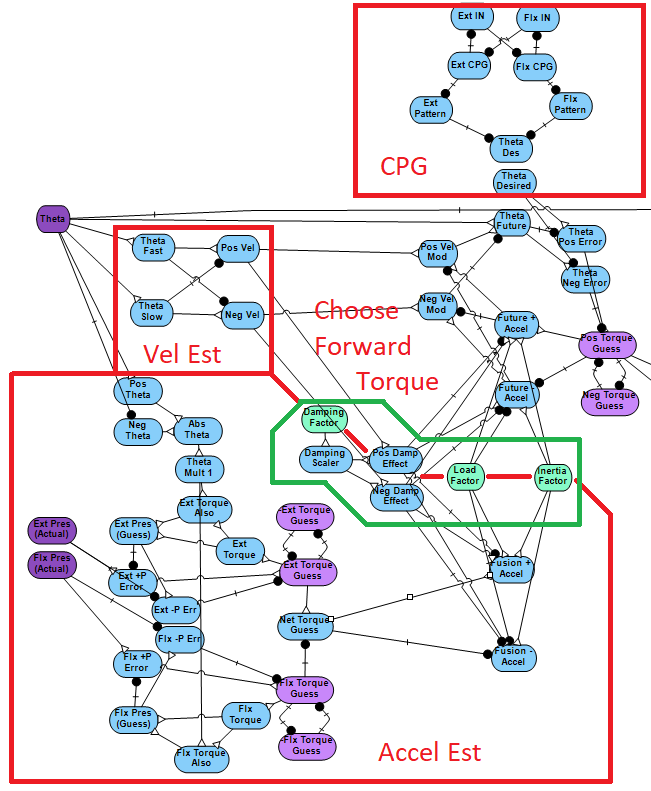
\includegraphics[height=5in, angle=0]{NetworkLayout}
\end{center}

The Inertia Factor (M) is connected via a division synapse. The Load Factor (N) is a signal transfer network. The Damping Factor (C) is connected via a multiplication synapse to modulate damping effects based on the sign of the velocity.

\bbs{What can I measure?}

The sensors on the robot measure position and pressures. From there, an estimation of velocity and acceleration can be obtained.

\begin{equation}
\ddot{\theta} = \dfrac{\tau - C \dot{\theta} - N}{M}
\end{equation}

\begin{equation}
\dot{\theta}_{1} = \dot{\theta}_{0} + \ddot{\theta} \delta t
\end{equation}

\begin{equation}
\dot{\theta}_{avg} = \dfrac{\dot{\theta}_{0} + \dot{\theta}_{1}}{2}
\end{equation}

\begin{equation}
\theta_{1} = \theta_{0} + \dot{\theta}_{avg} \delta t
\end{equation}

\bbss{Finding Error}

\bbsss{Acceleration Error}

\begin{equation}
\ddot{\theta}_{act} = \dfrac{\tau}{M} - \dfrac{C \dot{\theta}_{0}}{M} - \dfrac{N}{M}
\end{equation}

\begin{equation}
(\ddot{\theta}_{act} + \ddot{\theta}_{err}) = \dfrac{(\tau + \tau_{err})}{(M + M_{err})} - \dfrac{(C + C_{err}) (\dot{\theta}_{0} + \dot{\theta}_{err})}{(M + M_{err})} - \dfrac{(N + N_{err})}{(M + M_{err})}
\end{equation}

This equation includes some sources of error that are assumed to be small. This assumption may not be correct, but continued effort on estimation (in particular velocity estimation) will hope to minimize estimation errors (potentially by including concepts from Kalman filtering). Assumptions: no error in torque application, no error in velocity estimation and the mass/inertia is measured ahead of time.

The revised, simplified equation that assumes error comes from parameter estimation is as follows:

\begin{equation}
(\ddot{\theta}_{act} + \ddot{\theta}_{err}) = \dfrac{\tau}{M} - \dfrac{(C + C_{err})}{M}\dot{\theta}_{0} - \dfrac{(N + N_{err})}{M}
\end{equation}

With the correct/actual equation subtracted, the error components can be identified.

\begin{equation}
(\ddot{\theta}_{act} + \ddot{\theta}_{err}) - \ddot{\theta}_{act} =
\dfrac{\tau}{M} - \dfrac{\tau}{M}
- \dfrac{(C + C_{err})}{M}\dot{\theta}_{0} + \dfrac{C}{M}\dot{\theta}_{0}
- \dfrac{(N + N_{err})}{M}  + \dfrac{N}{M}
\end{equation}

\begin{equation}
\ddot{\theta}_{err} =
- C_{err} \dfrac{\dot{\theta}_{0}}{M}
- N_{err} \dfrac{1}{M}
\end{equation}

\begin{equation}
\ddot{\theta}_{err} = - \dfrac{1}{M}
(C_{err} \dot{\theta}_{0} + N_{err})
\end{equation}

For a known quantity of acceleration error $\ddot{\theta}_{err}$, there is a linear relation between $C_{err}$ and $N_{err}$, where $y = mx + b$.

\begin{equation}
N_{err} = 
- C_{err} \dot{\theta}_{0}
- M \ddot{\theta}_{err}
\end{equation}

$y = N_{err}$, $x = C_{err}$, $m = -\dot{\theta}$ and $b = - M \ddot{\theta}_{err}$. This gives a line of potential solutions and updates to each value where increasing $N_{err}$ leads to decreasing $C_{err}$ as expected. In order to pick a solution, the goal is chosen to minimize the squared update in C and N: minimize $F(C, N) = N_{err}^{2} + C_{err}^{2}$. This could be a useful exercise on its own, but there is additional information available in the form of velocity error and positional error.

\bbsss{Velocity Error}

\begin{equation}
(\dot{\theta}_{1, act} + \dot{\theta}_{1, err}) = \dot{\theta}_{0} + (\ddot{\theta}_{act} + \ddot{\theta}_{err}) \delta t
\end{equation}

\begin{equation}
\dot{\theta}_{1, err} = \ddot{\theta}_{err} \delta t
\end{equation}

\begin{equation}
\dot{\theta}_{1, err} = - \dfrac{\delta t}{M}(C_{err} \dot{\theta}_{0} + N_{err})
\end{equation}

\begin{equation}
(\dot{\theta}_{avg, act} + \dot{\theta}_{avg, err}) = \dfrac{\dot{\theta}_{0} + (\dot{\theta}_{1, act} + \dot{\theta}_{1, err})}{2}
\end{equation}

\begin{equation}
\dot{\theta}_{avg, err} = \dfrac{\dot{\theta}_{1, err}}{2}
\end{equation}

\begin{equation}
\dot{\theta}_{avg, err} = - \dfrac{\delta t}{2M}(C_{err} \dot{\theta}_{0} + N_{err}) = \dfrac{\delta t}{2} \ddot{\theta_{err}}
\end{equation}

\bbsss{Positional Error}

\begin{equation}
(\theta_{1, act} + \theta_{err}) = \theta_{0} + (\dot{\theta}_{avg} + \dot{\theta}_{avg, err}) \delta t
\end{equation}

\begin{equation}
\theta_{err} = \dot{\theta}_{avg, err} \delta t = \dfrac{\delta t^{2}}{2} \ddot{\theta_{err}} = - \dfrac{\delta t^{2}}{2M}(C_{err} \dot{\theta}_{0} + N_{err})
\end{equation}

\begin{equation}
- \dfrac{2M}{\delta t^{2}} \theta_{err} = C_{err} \dot{\theta}_{0} + N_{err}
\end{equation}

\begin{equation}
N_{err} = 
- \dot{\theta}_{0} C_{err}
- \dfrac{2M}{\delta t^{2}} \theta_{err}
\end{equation}

When $\dot{\theta}_{0}$ is 0, then $N_{err}$ explains the total error in acceleration. When $\dot{\theta}_{0}$ is large, $N_{err}$ should explain a diminishing ammount of the error. This can be thought of as finding the intersection between the given linear function and the vector $[\dot{\theta}_{0}, 1]$ scaled by a factor $\lambda$.

\begin{equation}
\lambda = 
- \lambda \dot{\theta}_{0}^{2}
- \dfrac{2M}{\delta t^{2}} \theta_{err}
\end{equation}

\begin{equation}
\lambda 
=
- \dfrac{2M}{\delta t^{2} (1 + \dot{\theta}_{0}^{2})} \theta_{err}
\end{equation}

\begin{equation}
C_{err} = \lambda \dot{\theta}, N_{err} = \lambda
\end{equation}

By following these steps, the updates for the Damping Factor and Load Factor can be updated ``easily". In neurons, $\dfrac{2}{\delta t^{2}}$ ammount to a scaling effect (the update rate is assumed constant) because the update will be modulated by a gain/moving average calculation so that single spurious measurements don't adversely impact stability. This leaves (with an arbitrary gain term $G$):

\begin{equation}
\lambda = G * (M * \theta_{err}) * \dfrac{1}{1 + \dot{\theta}^{2}}
\end{equation}

That last term looks like it will fit closely to a Signal Inverse Reduction (0.5x) synapse.

\end{document}
